\section{Related Libraries}
This section describes some libraries which come with \PGFPlots, but they are more or less special and need to be activated separately.
\pgfmanualpdflabel{\textbackslash usepgfplotslibrary}{}

\subsection{Dates as Input Coordinates}
\begin{pgfplotslibrary}{dateplot}
	A library which allows to use dates like |2008-01-01| or dates with time like |2008-01-01 11:35| as input coordinates in plots. The library converts dates to numbers and tick labels will be pretty-printed dates (or times).

	This library is documented in section~\ref{pgfplots:sec:symbolic:coords} on page~\pageref{pgfplots:sec:date:coords}.
\end{pgfplotslibrary}

\subsection{Clickable Plots}
\begin{pgfplotslibrary}{clickable}
	A library which generates small popups whenever one clicks into a plot. The popup displays the coordinate under the mouse pointer. Furthermore, the library allows to display slopes if one holds the mouse pressed and drags it to another point in the plot.


	It is completely sufficient to write 
\begin{codeexample}[code only]
\usepgfplotslibrary{clickable}
\end{codeexample}
	\noindent in the document preamble. This will automatically prepare every plot.

	The library works with Acrobat Javascript and \pdf\ forms: every plot becomes a push--button. 

	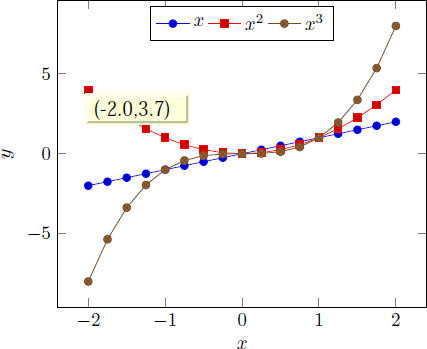
\includegraphics[height=6cm]{figures/pgfplotsclickable-fig1.png}
	\rlap{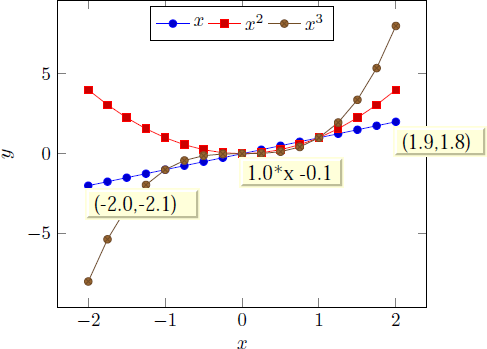
\includegraphics[height=6cm]{figures/pgfplotsclickable-fig2.png}}\hfill

	\nobreak
	These screen shots show the result of clicking into the axis range (left column) and of dragging from one point to another (right column). The second case shows the result of drag- and drop: it displays start- and end points and the equation for the line segment between between the first point of the drag- and drop and the second point where the mouse has been released. The line segment is 
	\[ l(x; x_0,y_0,x_1,y_1) = m \cdot x + n \]
	where $m = (y_1-y_0) / (x_1-x_0)$ is the slope and $n$ the offset chosen such that $l(x_0;\dotsc) = y_0$. For logarithmic plots, logarithms will be applied before computing slopes. 

	\noindent
	\hbox to \linewidth{%
	\hspace{-0.5cm}%
	\begin{tikzpicture}
		\node at (8cm,0cm)	{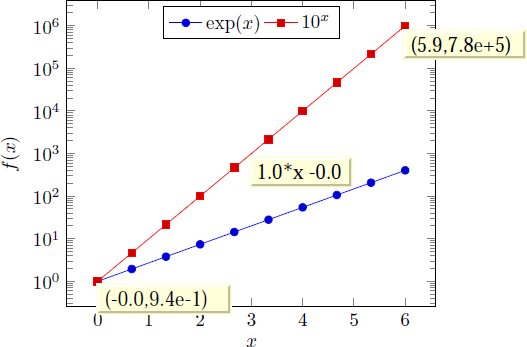
\includegraphics[height=6cm]{figures/pgfplotsclickable-fig4.png}};
		\node at (0cm,0cm)	{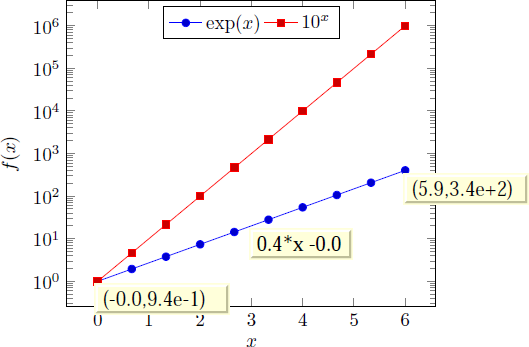
\includegraphics[height=6cm]{figures/pgfplotsclickable-fig3.png}};
	\end{tikzpicture}\hss}%

	\nobreak
	These screen shots show the result of drag- and drop for \emph{logarithmic} axes: the end points show, again, the coordinates (without logs) and the form field in the middle shows the slope and offset of the linear equation in log coordinates.

	The log basis for any logarithmic axes is usually~$10$, but it respects the current setting of |log basis x| and |log basis y|. The applied log will always use the same logarithm which is also used for the axis descriptions (this is not necessarily the same as used by \PGFPlotstable!).

	This document has been produced with the |clickable| library, so it is possible to load it into Acrobat Reader and simply click into a plot.
	
	\expandafter\ifx\csname pgfplotsclickabledisabled\endcsname\relax
	\else
	\paragraph{Attention:} For this document, the |clickable| library has been deactivated. You may find a different version on \url{http://sourceforge.net/projects/pgfplots}.
	\fi

	A click places an annotation at the coordinate under the mouse pointer, a snap--to--nearest feature is not available (yet?).

	\paragraph{Requirements:}
	\begin{itemize}
		\item The library relies on the \LaTeX\ packages |insdljs| (``Insert document level Javascript'') and |eforms| which are both part of the freely available |AcroTeX| education bundle~\cite{acrotex}\footnote{These packages rely on \LaTeX, so the library is only available for \LaTeX, not for plain \TeX\ or Con\TeX t.}. The |insdljs| package creates a temporary file with extension |.djs|.
		
		\item At the time of this writing, only Adobe Acrobat Reader interpretes Javascript and Forms properly. The library doesn't have any effect if the resulting document is used in other viewers (as far as I know).

	\end{itemize}
	Note that although this library has been written for \PGFPlots, it can be used independently of an \PGFPlots\ environment.

	\paragraph{Compatibility issues:}
	There a several restrictions when using this library. Most of them will vanish in future versions -- but up to now, I can't do magic.
	\begin{itemize}
		\item The library does not yet support rotated axes. Use |clickable=false| for those axes.
		\item The library works only with |pdflatex|, |dvips| or |dvipdfm| are not supported\footnote{In fact, they should be. I don't really know why they don't $\hdots$ any hint is welcome.}.

		\item Up to now, it is \emph{not} possible to use this library together with the |external| library and other image externalization methods of section~\ref{sec:pgfplots:importexport}.
		
		To be more precise, you can (with two extra preamble lines, see below) get correctly annotated, exported \pdf\ documents, but the |\includegraphics| command does not import the dynamic features.

		In case you decide to use this work--around, you need to insert
\begin{codeexample}[code only]
% \maxdeadcycles=10000 % in case you get the error `Output loop---<N> consecutive dead cycles.'
\usepackage[pdftex]{eforms}	
\end{codeexample}
		\noindent \emph{before} loading \pgfname, \Tikz\ or \PGFPlots. The |\maxdeadcycles| appears to be necessary for large documents, try it out.

		As long as you are working on a draft version of your document, you might want to use
\begin{codeexample}[code only]
\pgfkeys{/pgf/images/include external/.code={\href{file:#1}{\pgfimage{#1}}}
\end{codeexample}
		in your preamble. This will generate hyper links around the graphics files which link to the exported figures. Clicking on the hyper links opens the exported figure which, in turn, has been generated with the |clickable| library and allows dynamic features\footnote{This special treatment needs the external files in the same base directory as the main document, so this approach is most certainly \emph{not} suitable for a final document.}.


		\item The library automatically calls |\begin{Form}| at |\begin{document}| and |\end{Form}| at the end of the document. This environment of |hyperref| is necessary for dynamic user interaction and should be kept in mind if the document contains other form elements.
	\end{itemize}

	\paragraph{Acknowledgements:}
	\begin{itemize}
		\item I have used a javascript |sprintf| implementation of Kevin van Zonneveld~\cite{phptojs} (the javascript API has only a limited set of conversions).
	\end{itemize}
\end{pgfplotslibrary}

It is possible to customize |pgfplots.clickable| with several options.

\begin{pgfplotskey}{clickable=\mchoice{true,false} (initially true)}
	Allows to disable the library for single plots.
\end{pgfplotskey}

\begin{pgfplotskey}{annot/js fillColor=\marg{javascript color} (initially ["RGB",1,1,.855])}
	Sets the background (fill) color of the short popup annotations. 
	
	Possible choices are |transparent|, gray, RGB or CMYK color specified as four--element--arrays of the form
	|["RGB", |\meta{red}|,|\meta{green}|,|\meta{blue}|]|. Each color component is between $0$ and $1$.

	Again: this option is for Javascript. It is \emph{not} possible to use colors as in \pgfname.
\end{pgfplotskey}

\begin{pgfplotskey}{annot/point format=\marg{sprintf-format} (initially {(\%.1f,\%.1f)})}
	Allows to provide an |sprintf| format string which is used to fill the annotations with text. 
	The first argument to |sprintf| is the $x$-coordinate and the second argument is the $y$-coordinate.

	The |every semilogx axis|, |every semilogy axis| and |every loglog axis| styles have been updated to
\begin{codeexample}[code only]
\pgfplotsset{
	every semilogy axis/.append style={/pgfplots/annot/point format={(\%.1f,\%.1e)}},
	every semilogx axis/.append style={/pgfplots/annot/point format={(\%.1e,\%.1f)}},
	every loglog axis/.append style={/pgfplots/annot/point format={(\%.1e,\%.1e)}}
}
\end{codeexample}
	\noindent such that every logarithmic coordinate is displayed in scientific format.
\end{pgfplotskey}

\begin{pgfplotskey}{annot/slope format=\marg{sprintf-format} (initially \%.1f*x \%+.1f)}
	Allows to provide an |sprintf| format string which is used to fill the slope--annotation with text.
	The first argument is the slope and the second the line offset.
\end{pgfplotskey}

\begin{pgfplotskey}{annot/printable=\mchoice{true,false} (initially false)}
	Allows to configure whether the small annotations will be printed. Otherwise, they are only available on screen.
\end{pgfplotskey}

\begin{pgfplotskey}{annot/font=\marg{javascript font name} (initially font.Times)}
	Allows to choose a javascript font for the annotations. Possible choices are limited to what javascript accepts (which is \emph{not} the same as \LaTeX). The default fonts and its names are shown below.

	\begin{center}
	\begin{tabular}{ll}
		\toprule
		Font Name	& Name in Javascript\\
		\midrule
		Times-Roman           & font.Times\\
        Times-Bold            & font.TimesB\\
        Times-Italic          & font.TimesI\\
        Times-BoldItalic      & font.TimesBI\\
        Helvetica             & font.Helv\\
        Helvetica-Bold        & font.HelvB\\
        Helvetica-Oblique     & font.HelvI\\
        Helvetica-BoldOblique & font.HelvBI\\
        Courier               & font.Cour\\
        Courier-Bold          & font.CourB\\
        Courier-Oblique       & font.CourI\\
        Courier-BoldOblique   & font.CourBI\\
        Symbol                & font.Symbol\\
        ZapfDingbats          & font.ZapfD\\
		\bottomrule
	\end{tabular}
	\end{center}
\end{pgfplotskey}

\begin{pgfplotskey}{annot/textSize=\marg{Size in Point} (initially 11)}
	Sets the text size of annotations in points.
\end{pgfplotskey}

\subsubsection{Using the Clickable Library in Other Contexts}
This library provides essentially one command, |\pgfplotsclickablecreate| which creates a clickable area of predefined size, combined with javascript interaction code. It can be used independently of \PGFPlots.

\begin{command}{\pgfplotsclickablecreate\oarg{required key-value-options}}
	Creates an area which is clickable. A click produces a popup which
	contains information about the point under the cursor.
	
	The complete (!) context needs to be provided using key-value-pairs, either set before
	calling this method of inside of \oarg{required key-value-options}.
	
	This command actually creates an AcroForm which invokes javascript
	whenever it is clicked. A javascript Object is created which
	represents the context (axis limits and options). This javascript
	object is available at runtime.
	
	This method is public and it is \emph{not} restricted to \PGFPlots.
	The \PGFPlots\ hook simply initialises the required key-value-pairs.

	This method does not draw anything. It initialises only a
	clickable area and javascript code.
	
	The required key-value-pairs are documented below.
	
	\paragraph{Attention:} Complete key-value validation is \emph{not} performed here. It
	can happen that invalid options will produce javascript bugs when
	opened with Acrobat Reader. Use the javascript console to find them.
\end{command}

\noindent All options described in the following are only interesting for users who intend to use this library without \PGFPlots.

\begin{pgfplotskey}{annot/width=\marg{dimension} (initially -)}
	This required key communicates the area's width to |\pgfplotsclickablecreate|. It must be a \TeX\ dimension like |5cm|.
\end{pgfplotskey}
\begin{pgfplotskey}{annot/height=\marg{dimension} (initially -)}
	This required key communicates the area's height to |\pgfplotsclickablecreate|. It must be a \TeX\ dimension like |5cm|.
\end{pgfplotskey}
\begin{pgfplotskey}{annot/jsname=\marg{string} (initially -)}
	This required key communicates a unique identifier to |\pgfplotsclickablecreate|. This identifier is used to identify the object in javascript, so there can't be more than one of them. If it is empty, a default identifier will be created.
\end{pgfplotskey}

\begin{pgfplotskeylist}{annot/xmin=\marg{number},annot/xmax=\marg{number},annot/ymin=\marg{number},annot/ymax=\marg{number} (initially empty)}
	These required keys communicate the axis limits to |\pgfplotsclickablecreate|. They should be set to numbers which can be assigned to a javascript floating point number (standard IEEE double precision).
\end{pgfplotskeylist}

\input pgfplots.libs.units.tex
\input pgfplots.libs.groupplot.tex

\subsection{Image Externalization}
\begin{pgfplotslibrary}{external}
	The |external| library offers a convenient method to export every single |tikzpicture| into a separate~|.pdf| (or~|.eps|). Later runs of \LaTeX\ will simply include these graphics, thereby reducing typesetting time considerably.
	
	This library is documented in more detail in section~\ref{sec:pgfplots:export} ``Export to {\pdf/\eps}''.


	The |external| library has been written by Christian Feuers\"anger (author of \PGFPlots). It has been contributed to \Tikz\ as general purpose library, so the reference documentation along with all tweaks can be found in~\cite[Section ``Externalization Library'']{tikz}. The command |\usepgfplotslibrary{external}| is actually just a wrapper which loads |\usetikzlibrary{external}| or, if this library does not yet exist because the installed \pgfname\ has at most version $2.00$, it will load a copy which is shipped with \PGFPlots.
\end{pgfplotslibrary}
